%
%==> Section 1: What is TikZ?
%
\section{
  What is Ti$k$Z?
}

%
%==> What is TikZ
%
\begin{frame}
  \frametitle{
    What is Ti$k$Z?
  }
  \begin{enumerate}
  \item
    A recursive acronym for \textcolor{blue}{ \tt Ti$k$Z ist kein Zeichenprogramm} (German for ``Ti$k$Z is not a drawing program").
  \item
    More specifically, Ti$k$Z is a package for creating pictures.
  \item
    Create anything from rectangles, circles to Koch snowflakes, 3D graphs and animations.
  \item
    Ti$k$Z works very well with Beamer (they were written by the same person!). Muck thanks and gratitude to Till Tantau.
  \end{enumerate}

\end{frame}

%
%==> An image by Ben Cot\'e
%
\begin{frame} 
  \frametitle{
    An image by Ben Cot\'e
}
  
  {
    \tiny
    \begin{center}
      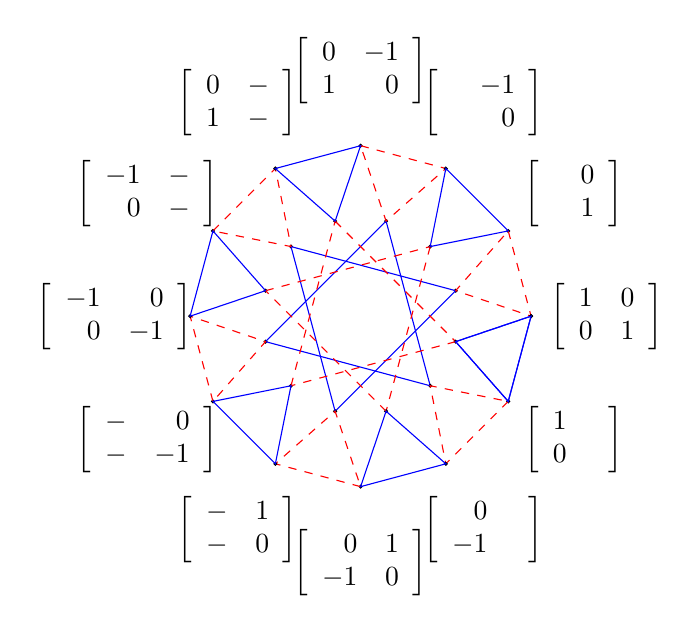
\begin{tikzpicture}[scale=1.25]
  \foreach \x in {15,75,...,330} {
    \filldraw[black] (\x:1cm) circle(0.4pt); % dots at each point
    % lines across inside
    \draw[blue] (\x:1cm) -- (\x-120:1cm);
  }
  \foreach \x in {45,105,...,345} {
    \filldraw[black] (\x:1cm) circle(0.4pt); % dots at each point
    % lines across outside
    \draw[red,dashed] (\x:1cm) -- (\x-120:1cm);
  }
  \foreach \x in {30,90,...,330} {
    \filldraw[black] (\x:1.73205cm) circle(0.4pt); % dots at each point
    % lines across inside
    \draw[red,dashed] (\x:1.73205cm) -- (\x-30:1.73205cm) -- (\x-15:1cm) -- cycle;
  }
  \foreach \x in  {0,60,...,360} {
    \filldraw[black] (\x:1.73205cm) circle(0.4pt); % dots at each point
    % lines across inside
    \draw[blue] (\x:1.73205cm) -- (\x-30:1.73205cm) -- (\x-15:1cm) -- cycle;
  }
  \foreach \x/\a/\b/\c/\d in {
    0/1/0/0/1,
    30/\ow/0/\w/1,
    60/\ow/-1/\w/0,
    90/0/-1/1/0,
    120/0/-\ow/1/-\w,
    150/-1/-\ow/0/-\w,
    180/-1/0/0/-1,
    210/-\ow/0/-\w/-1,
    240/-\ow/1/-\w/0,
    270/0/1/-1/0,
    300/0/\ow/-1/\w,
    330/1/\ow/0/\w
  }
  \draw (\x:2.5cm) node { $\left[ \begin{array}{rr} \a & \b \\  \c & \d \end{array}\right]$};      
\end{tikzpicture} 

    \end{center}
  }
  

\end{frame}

%
%==> Ben Cot\'e's source code
%
\begin{frame}[fragile]
  \frametitle{
    Ben Cot\'e's source code
  }

  {
    \tiny
    \lstinputlisting{./tex/src/image_by_ben.tex}
  }
  
\end{frame}

%
%==> Preliminaries
%
\begin{frame}[fragile]
  \frametitle{
    Preliminaries
  }

  \begin{enumerate}
  \item
    You need to add

    \begin{lstlisting}
      \usepackage{tikz}
    \end{lstlisting}

    to your document preamble. Other commands to put in preamble will be discussed later.
  \item
    When creating a picture use the {\tt tikzpicture} environment. E.g.

  \begin{lstlisting}
    \begin{tikzpicture}
      %
      %... code
      %
    \end{tikzpicture}
  \end{lstlisting}
  \end{enumerate}

\end{frame}
